\documentclass[journal, a4paper]{IEEEtran}

% some very useful LaTeX packages include:

%\usepackage{cite}      % Written by Donald Arseneau
                        % V1.6 and later of IEEEtran pre-defines the format
                        % of the cite.sty package \cite{} output to follow
                        % that of IEEE. Loading the cite package will
                        % result in citation numbers being automatically
                        % sorted and properly "ranged". i.e.,
                        % [1], [9], [2], [7], [5], [6]
                        % (without using cite.sty)
                        % will become:
                        % [1], [2], [5]--[7], [9] (using cite.sty)
                        % cite.sty's \cite will automatically add leading
                        % space, if needed. Use cite.sty's noadjust option
                        % (cite.sty V3.8 and later) if you want to turn this
                        % off. cite.sty is already installed on most LaTeX
                        % systems. The latest version can be obtained at:
                        % http://www.ctan.org/tex-archive/macros/latex/contrib/supported/cite/

\usepackage{graphicx}   % Written by David Carlisle and Sebastian Rahtz
                        % Required if you want graphics, photos, etc.
                        % graphicx.sty is already installed on most LaTeX
                        % systems. The latest version and documentation can
                        % be obtained at:
                        % http://www.ctan.org/tex-archive/macros/latex/required/graphics/
                        % Another good source of documentation is "Using
                        % Imported Graphics in LaTeX2e" by Keith Reckdahl
                        % which can be found as esplatex.ps and epslatex.pdf
                        % at: http://www.ctan.org/tex-archive/info/

%\usepackage{psfrag}    % Written by Craig Barratt, Michael C. Grant,
                        % and David Carlisle
                        % This package allows you to substitute LaTeX
                        % commands for text in imported EPS graphic files.
                        % In this way, LaTeX symbols can be placed into
                        % graphics that have been generated by other
                        % applications. You must use latex->dvips->ps2pdf
                        % workflow (not direct pdf output from pdflatex) if
                        % you wish to use this capability because it works
                        % via some PostScript tricks. Alternatively, the
                        % graphics could be processed as separate files via
                        % psfrag and dvips, then converted to PDF for
                        % inclusion in the main file which uses pdflatex.
                        % Docs are in "The PSfrag System" by Michael C. Grant
                        % and David Carlisle. There is also some information
                        % about using psfrag in "Using Imported Graphics in
                        % LaTeX2e" by Keith Reckdahl which documents the
                        % graphicx package (see above). The psfrag package
                        % and documentation can be obtained at:
                        % http://www.ctan.org/tex-archive/macros/latex/contrib/supported/psfrag/

%\usepackage{subfigure} % Written by Steven Douglas Cochran
                        % This package makes it easy to put subfigures
                        % in your figures. i.e., "figure 1a and 1b"
                        % Docs are in "Using Imported Graphics in LaTeX2e"
                        % by Keith Reckdahl which also documents the graphicx
                        % package (see above). subfigure.sty is already
                        % installed on most LaTeX systems. The latest version
                        % and documentation can be obtained at:
                        % http://www.ctan.org/tex-archive/macros/latex/contrib/supported/subfigure/

\usepackage{url}        % Written by Donald Arseneau
                        % Provides better support for handling and breaking
                        % URLs. url.sty is already installed on most LaTeX
                        % systems. The latest version can be obtained at:
                        % http://www.ctan.org/tex-archive/macros/latex/contrib/other/misc/
                        % Read the url.sty source comments for usage information.

%\usepackage{stfloats}  % Written by Sigitas Tolusis
                        % Gives LaTeX2e the ability to do double column
                        % floats at the bottom of the page as well as the top.
                        % (e.g., "\begin{figure*}[!b]" is not normally
                        % possible in LaTeX2e). This is an invasive package
                        % which rewrites many portions of the LaTeX2e output
                        % routines. It may not work with other packages that
                        % modify the LaTeX2e output routine and/or with other
                        % versions of LaTeX. The latest version and
                        % documentation can be obtained at:
                        % http://www.ctan.org/tex-archive/macros/latex/contrib/supported/sttools/
                        % Documentation is contained in the stfloats.sty
                        % comments as well as in the presfull.pdf file.
                        % Do not use the stfloats baselinefloat ability as
                        % IEEE does not allow \baselineskip to stretch.
                        % Authors submitting work to the IEEE should note
                        % that IEEE rarely uses double column equations and
                        % that authors should try to avoid such use.
                        % Do not be tempted to use the cuted.sty or
                        % midfloat.sty package (by the same author) as IEEE
                        % does not format its papers in such ways.

\usepackage{amsmath}    % From the American Mathematical Society
                        % A popular package that provides many helpful commands
                        % for dealing with mathematics. Note that the AMSmath
                        % package sets \interdisplaylinepenalty to 10000 thus
                        % preventing page breaks from occurring within multiline
                        % equations. Use:
%\interdisplaylinepenalty=2500
                        % after loading amsmath to restore such page breaks
                        % as IEEEtran.cls normally does. amsmath.sty is already
                        % installed on most LaTeX systems. The latest version
                        % and documentation can be obtained at:
                        % http://www.ctan.org/tex-archive/macros/latex/required/amslatex/math/
\usepackage{amssymb}
\usepackage{amsfonts} % for \mathbb
\usepackage{xfrac} % for \sfrac

% Other popular packages for formatting tables and equations include:

%\usepackage{array}
% Frank Mittelbach's and David Carlisle's array.sty which improves the
% LaTeX2e array and tabular environments to provide better appearances and
% additional user controls. array.sty is already installed on most systems.
% The latest version and documentation can be obtained at:
% http://www.ctan.org/tex-archive/macros/latex/required/tools/

% V1.6 of IEEEtran contains the IEEEeqnarray family of commands that can
% be used to generate multiline equations as well as matrices, tables, etc.

% Also of notable interest:
% Scott Pakin's eqparbox package for creating (automatically sized) equal
% width boxes. Available:
% http://www.ctan.org/tex-archive/macros/latex/contrib/supported/eqparbox/

% *** Do not adjust lengths that control margins, column widths, etc. ***
% *** Do not use packages that alter fonts (such as pslatex).         ***
% There should be no need to do such things with IEEEtran.cls V1.6 and later.


% Your document starts here!
\begin{document}

% Define document title and author
	\title{Forward Sensitivity Equations in the Presence of Events}
	\author{Daniel Kaschek and Matthew Fidler
	\thanks{}}
	\markboth{}{}
	\maketitle

% Write abstract here
\begin{abstract}
	Forward sensitivity equations are frequently used in optimization. Based on forward sensitivities, gradient and Hessian of the least squares function can be derived which allow to use gradient-based optimization methods. In the presence of events, i.e. sudden changes of the state variables, the differential equations and corresponding sensitivity equations are structurally unchanged. However, the events on states need to be accounted for as events in the sensitivities. Here, we derive these necessary events and present them in a way that helps with the implementation in computational software. Finally, the sensitivity events are illustrated on a typical example from pharmacometrics.
\end{abstract}

% Each section begins with a \section{title} command
\section{Introduction}
	% \PARstart{}{} creates a tall first letter for this first paragraph
	\PARstart{E}{vents} frequently are used in ODE systems.  These
	events include intervention events such as a dose
	or infusion, or process events like bile 
	dumping and gastric emptying.  These events change ordinary 
	differential equations (ODE) by changing its states.  Some of 
	the more interesting system events like zero order release, gastric 
	emptying and bioavailability are not known \emph{a-priori}.  Often these 
	events should be estimated from available data.
	
	Like many data-based estimation methods we may have an initial guess about
	when and how these events occur.  But we want to find the best solution
	by optimization to the data. This most often performed while trying to
	estimate some other processes and parameters of the ODE system. 
	
	Like many optimization problems with initial conditions, the system needs 
	to maximize the likelihood surface based on the next best step.  
	The directions to the best location is provided by the gradient.  
	With ODEs one way to calculate the is the forward sensitivity equations.
	
	Often when forward sensitivity analysis is calculated it is done without
	considering the events that are estimated.  This has been more often  handled by
	simple but inaccurate numerical derivatives, but less often by a formal
	sensitivity analysis (Ref).  A formal sensitivity analysis adds accuracy and often speeds up computation.
	
	Exact forward sensitivities of these events have been calculated, called jump sensitivities. These jump sensitivities depend on other events making it more difficult to calculate the forward sensitivity for these events easily in optimization.  In one optimization example, the next event time needs to be known before the event based sensitivities are calculated.
	
	However, a simple linearization allows the event sensitivities to depend only on the event itself.  This simplification adds minuscule to no loss in accuracy in the point derivative at the event time.  Additionally, this will also speed up computational time because the next event times do not need to be calculated for optimization.  The cost of this method is to introduce new events to the sensitivity states already calculated.
	
	Because of these advantages, we would like to share this new method of calculating jump sensitivities.
	

% Main Part
\section{Main Part}
\label{sec:main}
Let $\dot x = f(x, p, t)$ be a system of ordinary differential equations (ODEs) with the states $x(t) \in \mathbb R^n$, parameters $p \in \mathbb R^m$ and time $t \in \mathbb R$. The sensitivity equations corresponding to this dynamic system are
\begin{align}
\begin{aligned}
    \frac{d}{dt}\frac{\partial x_i}{\partial p_j} &= \frac{d}{dp_j} f_i(x, p, t)\\
        & = \frac{\partial f_i}{\partial x_k}\frac{\partial x_k}{\partial p_j} + 
            \frac{\partial f_i}{\partial p_j}.
\end{aligned}
 \label{eq:sens}
\end{align}
Let us assume that an event occurs at time $t_e$ that changes the current state vector $x(t_e)$ to the value $v_e \in \mathbb R^n$. Both $t_e$ and $v_e$ are assumed to be parameters for which sensitivities are to be determined.

Because changing $x(t_e)$ is a singular event in time, it does not change the structure of the ODEs. They are the same before and after the event time. Therefore, also the sensitivity equations, eq.~\eqref{eq:sens}, are structurally unchanged. However, the sensitivities themselves are affected by jumps at event time $t_e$, as being shown in this section.

The derivation is based on linearization of the ODE around $x(t_e) = x_e$, this is the value of $x(t)$ at the latest timepoint before the event occurs. With this choice, the linearized ODE reads
\begin{align}
    \dot x \doteq A(p, t) x + b(p, t)
    \label{eq:linearized}
\end{align}
with $A(p, t) = \left.\frac{\partial f}{\partial x}\right|_{x_e}(p, t)$ and $b(p, t) = f(x_e, p, t)- \left.\frac{\partial f}{\partial x}\right|_{x_e}(p, t)x_e$. The general solution of eq.~\eqref{eq:linearized} is
\begin{align}
    x(t) = \Phi(t)x_0 + \Phi(t)\int_0^t \Phi^{-1}(\tau)b(\tau)d\tau,\quad t\leq t_e,
    \label{eq:leqte}
\end{align}
where $\Phi(t) = \big(\varphi_1(t), \dots, \varphi_n(t)\big)$ is the matrix of linearly independent solutions $\varphi_i(t)$ of the homogeneous part of eq.~\eqref{eq:linearized}, i.e., $\forall i:\;\dot\varphi_i = A(p, t)\varphi_i$ with initial condition $\varphi_i(0) = {\rm e}_i$, the $i$'th unit vector. 

First, we note that the original and linearized ODE's have the same sensitivity equations. The jumps of the sensitivities that we derive based on eq.~\eqref{eq:linearized} are therefore valid for the sensitivities of the original ODE, too. Second, the solution after the event time $t_e$ can be explicitly stated as
\begin{align}
    x(t) = \Phi(t-t_e)v_e + \Phi(t)\int_{t_e}^{t}\Phi^{-1}(\tau)b(\tau)d\tau,\quad t > t_e.
    \label{eq:gte}
\end{align}

\subsection{Sensitivities with respect to $t_e$}
Based on the explicit solutions, eqs.~\eqref{eq:linearized} and \eqref{eq:gte}, we find that
\begin{align}
    \left.\frac{\partial x}{\partial t_e}\right|_{t = t_e} =
    \left\{
    \begin{array}{ll}
    0     & \textrm{, for } t\nearrow t_e \\
    -A v_e + \frac{\partial v_e}{\partial t_e} - b(t_e)     & \textrm{, for }t \searrow t_e, 
    \end{array}
    \right.
    \label{eq:jump}
\end{align}
where we have used that $\Phi(0) = \mathbb I$ is the unit matrix. The sensitivities with respect to $t_e$ jump at time point $t_e$. For $t > t_e$, the sensitivities propagate forward in time according to the sensitivity equations. The jump equation contains the derivative of $v_e$ which depends on the kind of the event.\\

\paragraph{Replacement} 
The value of the $i$'th state, $x_i$, is set to a predefined value $v_{e, i}$. In that case, the derivative vanishes and the sensitivity at time $t_e$ is
\begin{align}
    \lim_{t\searrow t_e}\frac{\partial x_i}{\partial t_e} = \left.\frac{\partial f_i}{\partial x}\right|_{x_e}\cdot (x_e - v_e) - f_i(x_e),
    \label{eq:replace}
\end{align}
where we have used the definition of $b(t_e)$. In the equation, $\cdot: \mathbb R^n\times \mathbb R^n\rightarrow \mathbb R$ denotes the scalar product. While the state value $x_i$ jumps, the other states $x_j$, $j\neq i$, are continued. Continuation means that $v_{e, j}$ is set to $x_{e, j}$ and we need eq.~\eqref{eq:leqte} evaluated at $t_e$ to get $\frac{\partial v_e}{\partial t_e} = Ax_e + b(t_e)$. The sensitivities become 
\begin{align}
    \lim_{t\searrow t_e}\frac{\partial x_j}{\partial t_e} = \left.\frac{\partial f_j}{\partial x}\right|_{x_e}\cdot (x_e - v_e).\label{eq:continued}
\end{align}
The contributions from $b$ cancel out. In conclusion, we find that an event at time $t_e$ affects sensitivities with respect to $t_e$ of both the affected and unaffected states.\\

\paragraph{Additive} 
A constant $\Delta x_i$ is added to the value of the $i$'th state, $x_i$. In that case, $v_e$ is set to eq.~\eqref{eq:leqte} evaluated at $t_e$ plus the constant $\Delta x_i$. Therefore, the same argumentation as in the continuated case holds and the sensitivity is the same as eq.~\eqref{eq:continued}. The Difference $x_e - v_e$ turns out to be either 0 (for the continued states) or $\Delta x_k$ (for the affected states $k$, in particular $k = i$).\\

\paragraph{Multiplicative}
The value of the $i$'th state, $x_i$, is multiplied with a constant $\alpha_i$. Eq.~\eqref{eq:continued} is evaluated at $t_e$ and multiplied by $\alpha$ to get $v_e$. Consequently, the derivative $\frac{\partial v_e}{\partial t_e}$ is computed and plugged into eq.~\eqref{eq:jump}, yielding
\begin{align}
    \lim_{t\searrow t_e}\frac{\partial x_i}{\partial t_e} = \left.\frac{\partial f_i}{\partial x}\right|_{x_e}\cdot (x_e - v_e) - (1-\alpha_i)f_i(x_e).
\end{align}
The difference $x_e - v_e$ is either 0 (for the continued states) or $(1-\alpha_k)x_{e, k}$ (for multiplied states).

\subsection{Sensitivities with respect to $v_e$}

% Derive sensitivities with respect to the jump value
We use again the explicit solutions eqs.~\eqref{eq:linearized} and \eqref{eq:gte} and find that
\begin{align}
    \left.\frac{\partial x}{\partial v_e}\right|_{t = t_e} =
    \left\{
    \begin{array}{ll}
    0     & \textrm{, for } t\nearrow t_e \\
    \mathbb I     & \textrm{, for }t \searrow t_e.
    \end{array}
    \right.
    \label{eq:value}
\end{align}
Again, the sensitivities jump. They are forward propagated according to their sensitivity equations. Based on eq.~\eqref{eq:value}, we can construct sensitivities in case of additive events, where $v_e = x_e + \Delta x$ with $\Delta x \in \mathbb R^n$, and multiplicative events, where $v_{e, i} = \alpha_i x_{e, i}$ with $i = 1, \dots, n$. This is:
\begin{align}
    \left.\frac{\partial x}{\partial \Delta x}\right|_{t = t_e} = \mathbb I, \qquad \left.\frac{\partial x}{\partial \alpha}\right|_{t = t_e} = {\rm diag}(x_e).
\end{align}

\subsection{Sensitivities with respect to $p$}

% Explain that also other sensitivities need to be reset

In the above sections we have derived expressions for the jumps of sensitivities with respect to event parameters. In this section we show that also sensitivities with respect to other parameters are affected by the events.

Let 
%$\frac{d}{dt}\frac{\partial x}{\partial p_j} = F_j(\frac{\partial x}{\partial p})$, $j = 1, \dots, m$, 
$S_j(t) = \frac{\partial x}{\partial p_j}(t) \in \mathbb R^n$
be the sensitivities with respect to $p_j$ as derived from the solution for $t \leq t_e$, eq.~\eqref{eq:leqte}. On the other hand, the right-sided limit $t\searrow t_e$ of $\frac{\partial x}{\partial p_j}$ as derived from eq.~\eqref{eq:gte} yields 
\begin{align}
    \lim_{t\searrow t_e}\frac{\partial x}{\partial p_j} = \frac{\partial v_e}{\partial p_j}.
    \label{eq:dxdp}
\end{align}
Based on eq.~\eqref{eq:dxdp} we construct sensitivities in case of replacement, additive, and multiplicative events. States $i$ which are set to $v_{e, i}$ by an event have $\lim_{t\searrow t_e}\frac{\partial x_i}{\partial p_j} = 0$. States $i$ affected by an additive event, $v_{e, i} = x_{e, i} + \Delta x_i$, have $\lim_{t\searrow t_e}\frac{\partial x_i}{\partial p_j} = \frac{\partial x_{e, i}}{\partial p_j} = S_{ij}(t_e)$, i.e., the sensitivities are continued. States~$i$ affected by a multiplicative event, $v_{e, i} = \alpha_i x_{e, i}$, have $\lim_{t\searrow t_e}\frac{\partial x_i}{\partial p_j} = \alpha_i S_{ij}(t_e)$, i.e., they are multiplied with the same constant $\alpha_i$ as the state value $x_i$.


\section{Implementation}

% Explain how to implement
% Each event of the form (var, time, value, method) triggers a
% sequence of events on the sensitivities. Derive this sequence
% of events for the three methods "replace", "add" and "multiply"

When working with events in numerical ODE solvers, events are typically defined in the format
\begin{center}
\begin{tabular}{|c|c|c|c|}\hline
     var & time & value & method \\
     \hline
\end{tabular}
\end{center}
where ``var'' denotes the state variable, ``time'' is the time point at which the event occurs, ``value'' is the event value and ``method'' is either replace, add or multiply.
	
Using the results from Section~\ref{sec:main} we are going to derive the set of events that apply for the sensitivities.

Without loss of generality, let ``var'' be $x_1$. The time and value parameters are denoted as $\tau$ and $\xi$, and the value be replaced. This event with the required additional events is shown in Table~\ref{tab:replacement}.
\begin{table}[ht]
\caption{Replacement event and list of required additional sensitivity events.}
\label{tab:replacement}
\begin{center}
\begin{tabular}{|r|l|l|l|l|}\hline
     1 & $x_1$ & $\tau$ & $\xi$ & replace \\
     \hline
     2 & $\sfrac{\partial x_1}{\partial p_j}$ & $\tau$ & $0$ & replace \\
     3 & $\sfrac{\partial x_1}{\partial \tau}$ & $\tau$ & $J_{11}(x_1-\xi)-f_1$ & add \\
     4 & $\sfrac{\partial x_k}{\partial \tau}$ & $\tau$ & $J_{k1}(x_1-\xi)$ & add \\
     5 &$\sfrac{\partial x_1}{\partial \xi}$ & $\tau$ & 1 & add \\
     \hline
\end{tabular}
\end{center}
\end{table}
In the table, $j$ ranges from 1 to $m$, $J_{11}$ denotes the (1, 1)-element of the Jacobian $J_{ij} = \lim\limits_{t \nearrow \tau}\frac{\partial f_i}{\partial x_j}(x(t), p, t)$ and $f_1$ denotes the first element of $f_i := \lim\limits_{t \nearrow \tau}f_i(x(t), p, t)$. Note that, depending on the numeric implementation of the events, the symbolic expressions for $J_{11}$ and $f_1$ can be used and evaluated within the event function based on the state values at the event time before execution of the event.

In case there are other events associated with the same event time parameter $\tau$ affecting other states $x_k$, the events in line~4 need to be added. Lines~3 and~4 have method = add because these contributions need to be accumulated. The summation taking place in this way corresponds to the scalar product found in eqs.~\eqref{eq:replace} and \eqref{eq:continued}.

In a similar way, we derive the table for additive events, see Table~\ref{tab:additive}.
\begin{table}[ht]
\caption{Additive event and list of required additional sensitivity events.}
\label{tab:additive}
\begin{center}
\begin{tabular}{|r|l|l|l|l|}\hline
     1 & $x_1$ & $\tau$ & $\delta$ & add \\
     \hline
     2 & $\sfrac{\partial x_1}{\partial p_j}$ & $\tau$ & $0$ & add \\
     3 & $\sfrac{\partial x_1}{\partial \tau}$ & $\tau$ & $J_{11}\delta$ & add \\
     4 & $\sfrac{\partial x_k}{\partial \tau}$ & $\tau$ & $J_{k1}\delta$ & add \\
     5 &$\sfrac{\partial x_1}{\partial \delta}$ & $\tau$ & 1 & add \\
     \hline
\end{tabular}
\end{center}
\end{table}
In the table, $\delta$ denotes the value which is added to $x_1$ at time $\tau$. The event in line~2 could be omitted. It is shown in the table to explicitly show that $\frac{\partial x_1}{\partial p_j}$ is not affected. The event in line~4 needs to be added if there are other events associated with the same time parameter $\tau$.

Finally, the table for multiplicative events is derived, see Table~\ref{tab:multi}.
\begin{table}[ht]
\caption{Multiplicative event and list of required additional sensitivity events.}
\label{tab:multi}
\begin{center}
\begin{tabular}{|r|l|l|l|l|}\hline
     1 & $x_1$ & $\tau$ & $\alpha$ & multiply \\
     \hline
     2 & $\sfrac{\partial x_1}{\partial p_j}$ & $\tau$ & $\alpha$ & multiply \\
     3 & $\sfrac{\partial x_1}{\partial \tau}$ & $\tau$ & $(1-\alpha)(J_{11}x_1-f_1)$ & add \\
     4 & $\sfrac{\partial x_k}{\partial \tau}$ & $\tau$ & $(1-\alpha)J_{k1}x_1$ & add \\
     5 &$\sfrac{\partial x_1}{\partial \alpha}$ & $\tau$ & $x_1$ & add \\
     \hline
\end{tabular}
\end{center}
\end{table}
In the table, $\alpha$ denotes the value by which $x_1$ is multiplied at time $\tau$. The event in line~4 needs to be added if there are other events associated with the same time parameter $\tau$.

\section{Example}

The event sensitivities are illustrated on a simple pharmacokinetic-pharmacodynamic (PK/PD) model. The PK and PD are described by a one compartment first order absorption model and an inhibitory IMAX model, respectively. The equations are
\begin{align}
  \frac{\rm d}{{\rm d}t}{\rm Ad} &= {\rm Favail}\cdot{\rm Input}-{\rm KA}\cdot{\rm Ad} \label{eq:ODE_1} \\ 
  \frac{\rm d}{{\rm d}t}{\rm Ac} &= {\rm KA}\cdot{\rm Ad}-\frac{\rm CL}{\rm V}{\rm Ac}\\
  \frac{\rm d}{{\rm d}t}{\rm Input} &= 0 \label{eq:ODE_3} \\
  {\rm Effect} &= {\rm E0}\cdot\left(1-\frac{\frac{\rm Ac}{\rm V}\cdot{\rm IMAX}}{{\rm IC50}+\frac{\rm Ac}{\rm V}}\right).\label{eq:effect}
\end{align}
All states and parameters are characterized in Table~\ref{tab:parameters}. 
\begin{table}[hb]
    \caption{Overview of model states and parameters.}
    \centering
    \begin{tabular}{l|l|c}
           & Description & (Initial) value \\
           \hline\hline
        Ad & Drug compartment & 0 \\
        Ac & Central compartment & 0\\
        Input & Dosing input & 0\\
        \hline
        Favail & Bioavailability & 1\\
        KA & Transfer rate & 1\\
        CL & Clearance rate & 6\\
        V & Central volume & 60\\
        E0 & Baseline effect & 15\\
        IMAX & Maximal inhibition & 1\\
        IC50 & Half maximal conc. & 1\\
        \hline
    \end{tabular}
    \label{tab:parameters}
\end{table}
The input is switched on and off by events:
\begin{center}
\begin{tabular}{|r|l|l|l|l|}\hline
     1 & Input & $\tau_1$ & $r_1$ & replace \\
     2 & Input & $\tau_2$ & 0 & replace\\
     \hline
\end{tabular}
\end{center}
Typically, the dosing is parameterized in terms of the lag time (tlag), the duration of the infusion (tinf) and the drug dose (dose). The event parameters $\tau_1$, $\tau_2$ and $r_1$ are expressed as functions of the dosing parameters:
\begin{align}
    \tau_1 = {\rm tlag},\quad \tau_2 = {\rm tlag} + {\rm tinf},\quad r_1 &= \frac{\rm dose}{\rm tinf},\label{eq:dosing}
\end{align}
with ${\rm tlag} = 10$, ${\rm tinf} = 10$, ${\rm dose} = 200$. The model, eqs.~(\ref{eq:ODE_1}--\ref{eq:ODE_3}), has been simulated between $t = 0$ and $t = 60$ alongside the sensitivity equations. Subsequently, the response in the effect compartment, eq.~\eqref{eq:effect}, was evaluated based on the solution of the ODE. To illustrate the event sensitivities, we computed derivatives of the Effect with respect to tlag, tinf and dose, where we used the chain rule to obtain expressions in terms of model sensitivities ($\sfrac{\rm dAc}{\rm d \tau_1}$, $\sfrac{\rm dAc}{\rm d \tau_2}$ and $\sfrac{\rm dAc}{{\rm d} r_1}$), and the Jacobian of the dosing parameterization, eq.~\eqref{eq:dosing}.

The simulation outcome is shown in Fig.~\ref{fig:simulation}. 
\begin{figure}[ht]
    \centering
    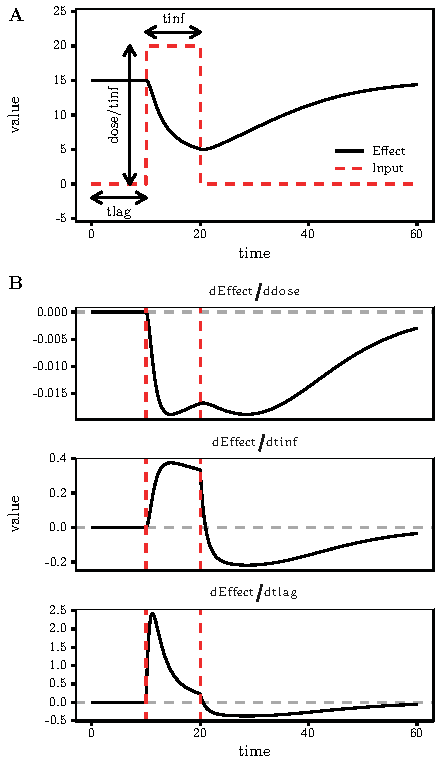
\includegraphics{example.pdf}
    \caption{Simulation of a PK/PD model. (A) The infusion input, parameterized by tlag, tinf and dose, provokes a response in the effect compartment. (B) The effect sensitivities with respect to the input parameters are shown. Start and end of the infusion are indicated by vertical dashed lines.}
    \label{fig:simulation}
\end{figure}
Upon dosing, the effect state is inhibited and recovers after the dosing input switches back to zero, shown in Fig.~\ref{fig:simulation}A. According to the effect sensitivities, see Fig.~\ref{fig:simulation}B, higher doses lead to stronger inhibition. A longer infusion time will decrease the inhibition during the infusion and increase it afterwards. The same holds for an increased lag time. The impact of the lag time is five times higher than the impact of the infusion time. The reason is that the infusion time is connected to the infusion rate $r_1$, i.e., a longer infusion time means a lower infusion rate to keep the dose constant.

Typically, the input is unobserved and the lag and infusion time need to be estimated from the observed effect. The derivatives $\frac{\rm dEffect}{\rm dtlag}$ and $\frac{\rm dEffect}{\rm dtinf}$ at the observation time points can be used to construct the gradient and Hessian of the least squares function. A typical application of the derivative $\frac{\rm dEffect}{\rm ddose}$ would be a sensitivity analysis.



\section{Conclusion}
	This section summarizes the paper.

% Now we need a bibliography:
% in this case 9, is the maximum number of references we expect
% put 99 if we have more than 9.
\begin{thebibliography}{9}

	%Each item starts with a \bibitem{reference} command and the details thereafter.
	\bibitem{Bar98}
	P.I.~Barton, R.J.~Allgor, W.F.~Feehery, and S.~Galán. Dynamic optimization in a discontinuous world. {\em Industrial \& Engineering Chemistry Research}, vol.~37, no.~3, pp.~966--981, Mar.~1998.
	
	\bibitem{Fro16}
	F.~Fr{\"o}hlich, F.~Theis, J.O.~R{\"a}dler, and J.~Hasenauer. Parameter estimation for dynamical systems with discrete events and logical operations. {\em Bioinformatics}, vol.~33, no.~7, pp.~1049--1056, Dec.~2016.
	
	
\end{thebibliography}

% Your document ends here!
\end{document}